% Created by tikzDevice version 0.12.3.1 on 2022-05-11 21:43:58
% !TEX encoding = UTF-8 Unicode
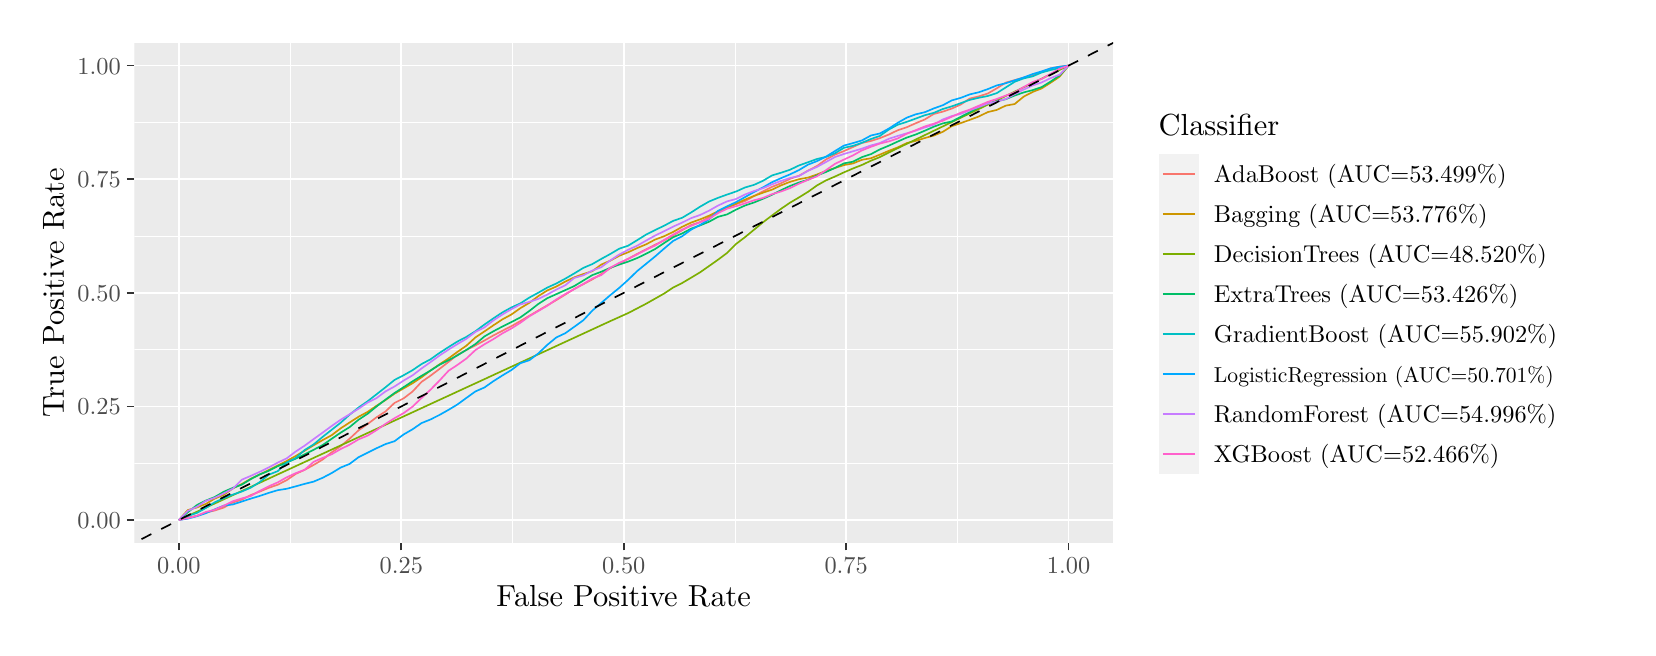
\begin{tikzpicture}[x=1pt,y=1pt]
\definecolor{fillColor}{RGB}{255,255,255}
\path[use as bounding box,fill=fillColor,fill opacity=0.00] (0,0) rectangle (578.16,216.81);
\begin{scope}
\path[clip] (  0.00,  0.00) rectangle (578.16,216.81);
\definecolor{drawColor}{RGB}{255,255,255}
\definecolor{fillColor}{RGB}{255,255,255}

\path[draw=drawColor,line width= 0.6pt,line join=round,line cap=round,fill=fillColor] (  0.00,  0.00) rectangle (578.16,216.81);
\end{scope}
\begin{scope}
\path[clip] ( 38.56, 30.69) rectangle (392.21,211.31);
\definecolor{fillColor}{gray}{0.92}

\path[fill=fillColor] ( 38.56, 30.69) rectangle (392.21,211.31);
\definecolor{drawColor}{RGB}{255,255,255}

\path[draw=drawColor,line width= 0.3pt,line join=round] ( 38.56, 59.42) --
	(392.21, 59.42);

\path[draw=drawColor,line width= 0.3pt,line join=round] ( 38.56,100.47) --
	(392.21,100.47);

\path[draw=drawColor,line width= 0.3pt,line join=round] ( 38.56,141.52) --
	(392.21,141.52);

\path[draw=drawColor,line width= 0.3pt,line join=round] ( 38.56,182.57) --
	(392.21,182.57);

\path[draw=drawColor,line width= 0.3pt,line join=round] ( 94.82, 30.69) --
	( 94.82,211.31);

\path[draw=drawColor,line width= 0.3pt,line join=round] (175.20, 30.69) --
	(175.20,211.31);

\path[draw=drawColor,line width= 0.3pt,line join=round] (255.57, 30.69) --
	(255.57,211.31);

\path[draw=drawColor,line width= 0.3pt,line join=round] (335.95, 30.69) --
	(335.95,211.31);

\path[draw=drawColor,line width= 0.6pt,line join=round] ( 38.56, 38.90) --
	(392.21, 38.90);

\path[draw=drawColor,line width= 0.6pt,line join=round] ( 38.56, 79.95) --
	(392.21, 79.95);

\path[draw=drawColor,line width= 0.6pt,line join=round] ( 38.56,121.00) --
	(392.21,121.00);

\path[draw=drawColor,line width= 0.6pt,line join=round] ( 38.56,162.05) --
	(392.21,162.05);

\path[draw=drawColor,line width= 0.6pt,line join=round] ( 38.56,203.10) --
	(392.21,203.10);

\path[draw=drawColor,line width= 0.6pt,line join=round] ( 54.63, 30.69) --
	( 54.63,211.31);

\path[draw=drawColor,line width= 0.6pt,line join=round] (135.01, 30.69) --
	(135.01,211.31);

\path[draw=drawColor,line width= 0.6pt,line join=round] (215.38, 30.69) --
	(215.38,211.31);

\path[draw=drawColor,line width= 0.6pt,line join=round] (295.76, 30.69) --
	(295.76,211.31);

\path[draw=drawColor,line width= 0.6pt,line join=round] (376.14, 30.69) --
	(376.14,211.31);
\definecolor{drawColor}{RGB}{248,118,109}

\path[draw=drawColor,line width= 0.6pt,line join=round] ( 54.63, 38.90) --
	( 57.88, 39.83) --
	( 61.13, 40.40) --
	( 64.37, 41.57) --
	( 67.62, 42.35) --
	( 70.87, 43.40) --
	( 74.12, 45.23) --
	( 77.36, 46.24) --
	( 80.61, 47.92) --
	( 83.86, 49.17) --
	( 87.11, 50.53) --
	( 90.35, 51.65) --
	( 93.60, 53.31) --
	( 96.85, 55.55) --
	(100.10, 57.04) --
	(103.34, 58.81) --
	(106.59, 60.74) --
	(109.84, 63.35) --
	(113.09, 65.55) --
	(116.33, 68.29) --
	(119.58, 71.32) --
	(122.83, 73.59) --
	(126.08, 76.03) --
	(129.32, 78.15) --
	(132.57, 81.22) --
	(135.82, 82.84) --
	(139.07, 85.32) --
	(142.31, 88.80) --
	(145.56, 91.04) --
	(148.81, 93.50) --
	(152.06, 96.02) --
	(155.30, 98.60) --
	(158.55,100.34) --
	(161.80,102.00) --
	(165.05,103.76) --
	(168.29,105.60) --
	(171.54,107.29) --
	(174.79,108.95) --
	(178.04,110.79) --
	(181.28,112.71) --
	(184.53,114.60) --
	(187.78,116.48) --
	(191.03,118.37) --
	(194.27,120.37) --
	(197.52,122.43) --
	(200.77,124.11) --
	(204.02,125.84) --
	(207.26,127.78) --
	(210.51,129.88) --
	(213.76,131.61) --
	(217.01,133.30) --
	(220.26,135.08) --
	(223.50,136.73) --
	(226.75,138.39) --
	(230.00,139.97) --
	(233.25,141.74) --
	(236.49,143.63) --
	(239.74,145.49) --
	(242.99,146.59) --
	(246.24,148.33) --
	(249.48,150.15) --
	(252.73,151.69) --
	(255.98,153.05) --
	(259.23,154.17) --
	(262.47,155.95) --
	(265.72,157.68) --
	(268.97,159.29) --
	(272.22,160.58) --
	(275.46,162.18) --
	(278.71,163.30) --
	(281.96,165.15) --
	(285.21,166.81) --
	(288.45,169.18) --
	(291.70,170.92) --
	(294.95,172.21) --
	(298.20,173.68) --
	(301.44,175.15) --
	(304.69,175.86) --
	(307.94,176.89) --
	(311.19,178.20) --
	(314.43,179.76) --
	(317.68,180.84) --
	(320.93,182.29) --
	(324.18,183.65) --
	(327.42,185.63) --
	(330.67,186.45) --
	(333.92,187.58) --
	(337.17,189.03) --
	(340.41,191.19) --
	(343.66,191.98) --
	(346.91,193.00) --
	(350.16,194.88) --
	(353.40,196.94) --
	(356.65,197.86) --
	(359.90,198.78) --
	(363.15,199.51) --
	(366.39,200.81) --
	(369.64,202.11) --
	(372.89,202.74) --
	(376.14,203.10);
\definecolor{drawColor}{RGB}{205,150,0}

\path[draw=drawColor,line width= 0.6pt,line join=round] ( 54.63, 38.90) --
	( 57.88, 42.49) --
	( 61.13, 43.43) --
	( 64.37, 44.71) --
	( 67.62, 46.65) --
	( 70.87, 47.99) --
	( 74.12, 50.31) --
	( 77.36, 51.91) --
	( 80.61, 53.81) --
	( 83.86, 55.37) --
	( 87.11, 56.99) --
	( 90.35, 58.59) --
	( 93.60, 60.24) --
	( 96.85, 62.04) --
	(100.10, 63.95) --
	(103.34, 65.92) --
	(106.59, 67.78) --
	(109.84, 69.55) --
	(113.09, 72.02) --
	(116.33, 74.14) --
	(119.58, 76.22) --
	(122.83, 77.97) --
	(126.08, 80.19) --
	(129.32, 82.27) --
	(132.57, 84.55) --
	(135.82, 86.45) --
	(139.07, 88.32) --
	(142.31, 90.47) --
	(145.56, 92.93) --
	(148.81, 95.14) --
	(152.06, 97.28) --
	(155.30, 99.66) --
	(158.55,101.91) --
	(161.80,104.88) --
	(165.05,107.04) --
	(168.29,109.26) --
	(171.54,111.40) --
	(174.79,113.16) --
	(178.04,115.46) --
	(181.28,117.39) --
	(184.53,119.81) --
	(187.78,121.86) --
	(191.03,123.27) --
	(194.27,125.07) --
	(197.52,126.59) --
	(200.77,127.79) --
	(204.02,128.80) --
	(207.26,131.20) --
	(210.51,132.60) --
	(213.76,134.38) --
	(217.01,135.67) --
	(220.26,137.17) --
	(223.50,138.54) --
	(226.75,140.25) --
	(230.00,141.45) --
	(233.25,143.01) --
	(236.49,144.84) --
	(239.74,146.38) --
	(242.99,147.54) --
	(246.24,148.88) --
	(249.48,150.46) --
	(252.73,151.70) --
	(255.98,153.21) --
	(259.23,154.69) --
	(262.47,156.01) --
	(265.72,157.18) --
	(268.97,158.27) --
	(272.22,159.82) --
	(275.46,161.09) --
	(278.71,162.05) --
	(281.96,162.64) --
	(285.21,163.75) --
	(288.45,165.06) --
	(291.70,166.09) --
	(294.95,167.15) --
	(298.20,167.74) --
	(301.44,169.06) --
	(304.69,169.62) --
	(307.94,170.93) --
	(311.19,172.31) --
	(314.43,173.57) --
	(317.68,175.11) --
	(320.93,175.92) --
	(324.18,176.93) --
	(327.42,177.82) --
	(330.67,179.17) --
	(333.92,181.22) --
	(337.17,182.32) --
	(340.41,183.49) --
	(343.66,184.70) --
	(346.91,186.30) --
	(350.16,187.08) --
	(353.40,188.63) --
	(356.65,189.22) --
	(359.90,191.89) --
	(363.15,193.57) --
	(366.39,194.86) --
	(369.64,196.91) --
	(372.89,199.11) --
	(376.14,203.10);
\definecolor{drawColor}{RGB}{124,174,0}

\path[draw=drawColor,line width= 0.6pt,line join=round] ( 54.63, 38.90) --
	( 57.88, 40.39) --
	( 61.13, 41.89) --
	( 64.37, 43.39) --
	( 67.62, 44.88) --
	( 70.87, 46.38) --
	( 74.12, 47.88) --
	( 77.36, 49.38) --
	( 80.61, 50.87) --
	( 83.86, 52.37) --
	( 87.11, 53.87) --
	( 90.35, 55.37) --
	( 93.60, 56.86) --
	( 96.85, 58.36) --
	(100.10, 59.86) --
	(103.34, 61.35) --
	(106.59, 62.85) --
	(109.84, 64.35) --
	(113.09, 65.85) --
	(116.33, 67.34) --
	(119.58, 68.84) --
	(122.83, 70.34) --
	(126.08, 71.84) --
	(129.32, 73.33) --
	(132.57, 74.83) --
	(135.82, 76.33) --
	(139.07, 77.82) --
	(142.31, 79.32) --
	(145.56, 80.82) --
	(148.81, 82.32) --
	(152.06, 83.81) --
	(155.30, 85.31) --
	(158.55, 86.81) --
	(161.80, 88.30) --
	(165.05, 89.80) --
	(168.29, 91.30) --
	(171.54, 92.80) --
	(174.79, 94.29) --
	(178.04, 95.79) --
	(181.28, 97.29) --
	(184.53, 98.79) --
	(187.78,100.28) --
	(191.03,101.78) --
	(194.27,103.28) --
	(197.52,104.77) --
	(200.77,106.27) --
	(204.02,107.77) --
	(207.26,109.27) --
	(210.51,110.76) --
	(213.76,112.23) --
	(217.01,113.69) --
	(220.26,115.38) --
	(223.50,117.07) --
	(226.75,118.91) --
	(230.00,120.75) --
	(233.25,122.92) --
	(236.49,124.54) --
	(239.74,126.46) --
	(242.99,128.42) --
	(246.24,130.69) --
	(249.48,132.98) --
	(252.73,135.41) --
	(255.98,138.66) --
	(259.23,141.13) --
	(262.47,143.80) --
	(265.72,146.49) --
	(268.97,148.95) --
	(272.22,151.35) --
	(275.46,153.56) --
	(278.71,155.47) --
	(281.96,157.48) --
	(285.21,159.80) --
	(288.45,161.61) --
	(291.70,163.01) --
	(294.95,164.52) --
	(298.20,165.92) --
	(301.44,167.19) --
	(304.69,168.73) --
	(307.94,170.04) --
	(311.19,171.70) --
	(314.43,173.27) --
	(317.68,174.84) --
	(320.93,176.41) --
	(324.18,177.98) --
	(327.42,179.55) --
	(330.67,181.12) --
	(333.92,182.69) --
	(337.17,184.26) --
	(340.41,185.83) --
	(343.66,187.40) --
	(346.91,188.97) --
	(350.16,190.54) --
	(353.40,192.11) --
	(356.65,193.68) --
	(359.90,195.25) --
	(363.15,196.82) --
	(366.39,198.39) --
	(369.64,199.96) --
	(372.89,201.53) --
	(376.14,203.10);
\definecolor{drawColor}{RGB}{0,190,103}

\path[draw=drawColor,line width= 0.6pt,line join=round] ( 54.63, 38.90) --
	( 57.88, 41.71) --
	( 61.13, 44.28) --
	( 64.37, 45.91) --
	( 67.62, 47.23) --
	( 70.87, 49.12) --
	( 74.12, 50.52) --
	( 77.36, 51.67) --
	( 80.61, 53.68) --
	( 83.86, 55.38) --
	( 87.11, 56.68) --
	( 90.35, 58.35) --
	( 93.60, 59.67) --
	( 96.85, 61.07) --
	(100.10, 62.65) --
	(103.34, 64.29) --
	(106.59, 65.98) --
	(109.84, 68.25) --
	(113.09, 70.46) --
	(116.33, 72.47) --
	(119.58, 75.16) --
	(122.83, 77.29) --
	(126.08, 79.94) --
	(129.32, 82.43) --
	(132.57, 84.80) --
	(135.82, 86.89) --
	(139.07, 89.02) --
	(142.31, 91.00) --
	(145.56, 92.90) --
	(148.81, 95.00) --
	(152.06, 96.62) --
	(155.30, 98.41) --
	(158.55,100.39) --
	(161.80,102.49) --
	(165.05,105.24) --
	(168.29,107.10) --
	(171.54,108.81) --
	(174.79,110.42) --
	(178.04,112.12) --
	(181.28,114.44) --
	(184.53,116.98) --
	(187.78,119.06) --
	(191.03,120.52) --
	(194.27,121.97) --
	(197.52,123.45) --
	(200.77,125.43) --
	(204.02,127.39) --
	(207.26,128.61) --
	(210.51,130.03) --
	(213.76,131.21) --
	(217.01,132.28) --
	(220.26,133.56) --
	(223.50,135.15) --
	(226.75,136.82) --
	(230.00,139.00) --
	(233.25,141.09) --
	(236.49,142.45) --
	(239.74,144.19) --
	(242.99,145.36) --
	(246.24,146.69) --
	(249.48,148.46) --
	(252.73,149.33) --
	(255.98,151.06) --
	(259.23,152.56) --
	(262.47,153.64) --
	(265.72,154.98) --
	(268.97,156.42) --
	(272.22,158.08) --
	(275.46,159.60) --
	(278.71,160.86) --
	(281.96,161.86) --
	(285.21,163.41) --
	(288.45,164.65) --
	(291.70,166.11) --
	(294.95,167.78) --
	(298.20,168.37) --
	(301.44,170.02) --
	(304.69,171.10) --
	(307.94,172.82) --
	(311.19,174.18) --
	(314.43,175.67) --
	(317.68,177.10) --
	(320.93,178.22) --
	(324.18,179.58) --
	(327.42,181.02) --
	(330.67,182.22) --
	(333.92,182.91) --
	(337.17,184.60) --
	(340.41,186.25) --
	(343.66,188.07) --
	(346.91,189.40) --
	(350.16,190.22) --
	(353.40,190.96) --
	(356.65,192.28) --
	(359.90,193.41) --
	(363.15,194.24) --
	(366.39,195.32) --
	(369.64,197.34) --
	(372.89,199.55) --
	(376.14,203.10);
\definecolor{drawColor}{RGB}{0,191,196}

\path[draw=drawColor,line width= 0.6pt,line join=round] ( 54.63, 38.90) --
	( 57.88, 40.37) --
	( 61.13, 41.44) --
	( 64.37, 43.25) --
	( 67.62, 45.32) --
	( 70.87, 46.79) --
	( 74.12, 48.08) --
	( 77.36, 49.19) --
	( 80.61, 50.58) --
	( 83.86, 52.61) --
	( 87.11, 55.28) --
	( 90.35, 56.55) --
	( 93.60, 59.67) --
	( 96.85, 61.33) --
	(100.10, 64.20) --
	(103.34, 66.23) --
	(106.59, 68.95) --
	(109.84, 71.50) --
	(113.09, 74.05) --
	(116.33, 76.95) --
	(119.58, 79.57) --
	(122.83, 81.81) --
	(126.08, 84.35) --
	(129.32, 86.88) --
	(132.57, 89.52) --
	(135.82, 91.20) --
	(139.07, 93.04) --
	(142.31, 95.25) --
	(145.56, 96.97) --
	(148.81, 99.28) --
	(152.06,101.38) --
	(155.30,103.41) --
	(158.55,105.09) --
	(161.80,107.12) --
	(165.05,109.54) --
	(168.29,111.77) --
	(171.54,113.92) --
	(174.79,115.71) --
	(178.04,117.18) --
	(181.28,119.28) --
	(184.53,121.04) --
	(187.78,122.89) --
	(191.03,124.38) --
	(194.27,126.12) --
	(197.52,128.01) --
	(200.77,130.00) --
	(204.02,131.38) --
	(207.26,133.24) --
	(210.51,135.02) --
	(213.76,136.94) --
	(217.01,138.05) --
	(220.26,140.03) --
	(223.50,142.06) --
	(226.75,143.70) --
	(230.00,145.25) --
	(233.25,147.00) --
	(236.49,148.11) --
	(239.74,150.04) --
	(242.99,152.13) --
	(246.24,154.00) --
	(249.48,155.33) --
	(252.73,156.51) --
	(255.98,157.61) --
	(259.23,159.07) --
	(262.47,160.01) --
	(265.72,161.49) --
	(268.97,163.42) --
	(272.22,164.39) --
	(275.46,165.47) --
	(278.71,167.02) --
	(281.96,168.18) --
	(285.21,169.36) --
	(288.45,170.11) --
	(291.70,171.42) --
	(294.95,173.39) --
	(298.20,174.10) --
	(301.44,175.20) --
	(304.69,176.57) --
	(307.94,177.69) --
	(311.19,180.00) --
	(314.43,181.75) --
	(317.68,182.78) --
	(320.93,183.97) --
	(324.18,185.17) --
	(327.42,186.02) --
	(330.67,187.41) --
	(333.92,188.37) --
	(337.17,189.54) --
	(340.41,190.71) --
	(343.66,191.47) --
	(346.91,192.11) --
	(350.16,193.15) --
	(353.40,195.19) --
	(356.65,197.25) --
	(359.90,198.47) --
	(363.15,199.23) --
	(366.39,200.61) --
	(369.64,201.50) --
	(372.89,202.23) --
	(376.14,203.10);
\definecolor{drawColor}{RGB}{0,169,255}

\path[draw=drawColor,line width= 0.6pt,line join=round] ( 54.63, 38.90) --
	( 57.88, 39.40) --
	( 61.13, 40.27) --
	( 64.37, 41.36) --
	( 67.62, 42.76) --
	( 70.87, 44.11) --
	( 74.12, 44.52) --
	( 77.36, 45.56) --
	( 80.61, 46.63) --
	( 83.86, 47.60) --
	( 87.11, 48.71) --
	( 90.35, 49.68) --
	( 93.60, 50.19) --
	( 96.85, 51.06) --
	(100.10, 51.97) --
	(103.34, 52.78) --
	(106.59, 54.16) --
	(109.84, 55.86) --
	(113.09, 57.85) --
	(116.33, 59.17) --
	(119.58, 61.62) --
	(122.83, 63.21) --
	(126.08, 64.84) --
	(129.32, 66.34) --
	(132.57, 67.38) --
	(135.82, 69.80) --
	(139.07, 71.68) --
	(142.31, 73.92) --
	(145.56, 75.24) --
	(148.81, 76.87) --
	(152.06, 78.70) --
	(155.30, 80.66) --
	(158.55, 83.03) --
	(161.80, 85.37) --
	(165.05, 86.79) --
	(168.29, 89.07) --
	(171.54, 91.13) --
	(174.79, 93.09) --
	(178.04, 95.57) --
	(181.28, 96.64) --
	(184.53, 99.11) --
	(187.78,102.20) --
	(191.03,104.88) --
	(194.27,106.40) --
	(197.52,108.72) --
	(200.77,111.07) --
	(204.02,114.55) --
	(207.26,117.35) --
	(210.51,120.14) --
	(213.76,122.79) --
	(217.01,125.72) --
	(220.26,128.87) --
	(223.50,131.51) --
	(226.75,134.16) --
	(230.00,137.00) --
	(233.25,139.75) --
	(236.49,141.44) --
	(239.74,143.81) --
	(242.99,145.55) --
	(246.24,147.55) --
	(249.48,150.63) --
	(252.73,152.25) --
	(255.98,153.78) --
	(259.23,155.59) --
	(262.47,157.44) --
	(265.72,159.10) --
	(268.97,160.98) --
	(272.22,162.43) --
	(275.46,163.80) --
	(278.71,165.35) --
	(281.96,167.31) --
	(285.21,168.58) --
	(288.45,170.19) --
	(291.70,172.22) --
	(294.95,174.20) --
	(298.20,175.09) --
	(301.44,176.06) --
	(304.69,177.84) --
	(307.94,178.58) --
	(311.19,180.36) --
	(314.43,182.45) --
	(317.68,184.30) --
	(320.93,185.51) --
	(324.18,186.26) --
	(327.42,187.63) --
	(330.67,188.78) --
	(333.92,190.53) --
	(337.17,191.45) --
	(340.41,192.70) --
	(343.66,193.46) --
	(346.91,194.60) --
	(350.16,195.93) --
	(353.40,196.72) --
	(356.65,197.76) --
	(359.90,198.83) --
	(363.15,200.05) --
	(366.39,201.02) --
	(369.64,202.11) --
	(372.89,202.69) --
	(376.14,203.10);
\definecolor{drawColor}{RGB}{199,124,255}

\path[draw=drawColor,line width= 0.6pt,line join=round] ( 54.63, 38.90) --
	( 57.88, 42.21) --
	( 61.13, 43.68) --
	( 64.37, 45.79) --
	( 67.62, 46.94) --
	( 70.87, 48.53) --
	( 74.12, 50.23) --
	( 77.36, 53.47) --
	( 80.61, 54.84) --
	( 83.86, 56.32) --
	( 87.11, 57.90) --
	( 90.35, 59.63) --
	( 93.60, 61.18) --
	( 96.85, 63.64) --
	(100.10, 65.78) --
	(103.34, 68.15) --
	(106.59, 70.49) --
	(109.84, 72.87) --
	(113.09, 75.13) --
	(116.33, 77.12) --
	(119.58, 79.12) --
	(122.83, 81.33) --
	(126.08, 82.97) --
	(129.32, 85.39) --
	(132.57, 87.15) --
	(135.82, 89.27) --
	(139.07, 91.18) --
	(142.31, 93.65) --
	(145.56, 95.96) --
	(148.81, 98.32) --
	(152.06,100.48) --
	(155.30,102.48) --
	(158.55,104.40) --
	(161.80,106.86) --
	(165.05,108.52) --
	(168.29,111.02) --
	(171.54,113.16) --
	(174.79,115.09) --
	(178.04,116.80) --
	(181.28,117.74) --
	(184.53,118.81) --
	(187.78,120.37) --
	(191.03,122.18) --
	(194.27,123.73) --
	(197.52,126.38) --
	(200.77,127.31) --
	(204.02,129.03) --
	(207.26,130.25) --
	(210.51,132.70) --
	(213.76,134.84) --
	(217.01,136.56) --
	(220.26,138.04) --
	(223.50,139.89) --
	(226.75,141.71) --
	(230.00,143.27) --
	(233.25,144.92) --
	(236.49,146.37) --
	(239.74,147.99) --
	(242.99,149.13) --
	(246.24,150.69) --
	(249.48,152.54) --
	(252.73,154.04) --
	(255.98,154.90) --
	(259.23,156.53) --
	(262.47,157.79) --
	(265.72,158.79) --
	(268.97,160.19) --
	(272.22,161.44) --
	(275.46,162.49) --
	(278.71,163.19) --
	(281.96,165.07) --
	(285.21,166.49) --
	(288.45,168.25) --
	(291.70,170.06) --
	(294.95,171.17) --
	(298.20,172.13) --
	(301.44,173.10) --
	(304.69,174.25) --
	(307.94,175.12) --
	(311.19,176.66) --
	(314.43,177.70) --
	(317.68,178.65) --
	(320.93,179.61) --
	(324.18,180.74) --
	(327.42,181.75) --
	(330.67,183.65) --
	(333.92,184.86) --
	(337.17,185.66) --
	(340.41,186.94) --
	(343.66,188.15) --
	(346.91,189.38) --
	(350.16,190.09) --
	(353.40,191.03) --
	(356.65,192.79) --
	(359.90,194.44) --
	(363.15,195.94) --
	(366.39,197.02) --
	(369.64,198.57) --
	(372.89,199.82) --
	(376.14,203.10);
\definecolor{drawColor}{RGB}{255,97,204}

\path[draw=drawColor,line width= 0.6pt,line join=round] ( 54.63, 38.90) --
	( 57.88, 39.58) --
	( 61.13, 40.40) --
	( 64.37, 41.80) --
	( 67.62, 42.61) --
	( 70.87, 44.08) --
	( 74.12, 45.69) --
	( 77.36, 46.70) --
	( 80.61, 47.57) --
	( 83.86, 49.45) --
	( 87.11, 51.08) --
	( 90.35, 52.50) --
	( 93.60, 54.33) --
	( 96.85, 55.83) --
	(100.10, 57.06) --
	(103.34, 59.93) --
	(106.59, 61.35) --
	(109.84, 62.65) --
	(113.09, 64.54) --
	(116.33, 66.12) --
	(119.58, 68.05) --
	(122.83, 69.39) --
	(126.08, 71.39) --
	(129.32, 73.65) --
	(132.57, 75.70) --
	(135.82, 77.51) --
	(139.07, 79.87) --
	(142.31, 82.97) --
	(145.56, 85.99) --
	(148.81, 89.29) --
	(152.06, 92.81) --
	(155.30, 94.96) --
	(158.55, 97.28) --
	(161.80,100.32) --
	(165.05,102.40) --
	(168.29,104.27) --
	(171.54,106.34) --
	(174.79,108.11) --
	(178.04,110.18) --
	(181.28,112.51) --
	(184.53,114.42) --
	(187.78,116.34) --
	(191.03,118.61) --
	(194.27,120.57) --
	(197.52,122.33) --
	(200.77,124.20) --
	(204.02,126.15) --
	(207.26,127.40) --
	(210.51,130.07) --
	(213.76,131.82) --
	(217.01,133.27) --
	(220.26,134.90) --
	(223.50,136.57) --
	(226.75,138.09) --
	(230.00,140.13) --
	(233.25,142.05) --
	(236.49,143.86) --
	(239.74,145.21) --
	(242.99,146.51) --
	(246.24,147.77) --
	(249.48,149.81) --
	(252.73,151.39) --
	(255.98,152.30) --
	(259.23,153.32) --
	(262.47,154.44) --
	(265.72,155.29) --
	(268.97,156.65) --
	(272.22,157.62) --
	(275.46,158.82) --
	(278.71,160.43) --
	(281.96,161.81) --
	(285.21,163.11) --
	(288.45,165.30) --
	(291.70,167.59) --
	(294.95,169.14) --
	(298.20,170.65) --
	(301.44,172.46) --
	(304.69,173.75) --
	(307.94,174.92) --
	(311.19,175.73) --
	(314.43,176.80) --
	(317.68,178.48) --
	(320.93,179.78) --
	(324.18,181.12) --
	(327.42,182.12) --
	(330.67,183.16) --
	(333.92,184.63) --
	(337.17,186.08) --
	(340.41,187.20) --
	(343.66,188.60) --
	(346.91,189.97) --
	(350.16,191.04) --
	(353.40,192.26) --
	(356.65,193.43) --
	(359.90,195.34) --
	(363.15,197.15) --
	(366.39,198.27) --
	(369.64,200.12) --
	(372.89,202.01) --
	(376.14,203.10);
\definecolor{drawColor}{RGB}{0,0,0}

\path[draw=drawColor,line width= 0.6pt,dash pattern=on 4pt off 4pt ,line join=round] (-315.10,-149.94) -- (745.87,391.93);
\end{scope}
\begin{scope}
\path[clip] (  0.00,  0.00) rectangle (578.16,216.81);
\definecolor{drawColor}{gray}{0.30}

\node[text=drawColor,anchor=base east,inner sep=0pt, outer sep=0pt, scale=  0.88] at ( 33.61, 35.87) {0.00};

\node[text=drawColor,anchor=base east,inner sep=0pt, outer sep=0pt, scale=  0.88] at ( 33.61, 76.92) {0.25};

\node[text=drawColor,anchor=base east,inner sep=0pt, outer sep=0pt, scale=  0.88] at ( 33.61,117.97) {0.50};

\node[text=drawColor,anchor=base east,inner sep=0pt, outer sep=0pt, scale=  0.88] at ( 33.61,159.02) {0.75};

\node[text=drawColor,anchor=base east,inner sep=0pt, outer sep=0pt, scale=  0.88] at ( 33.61,200.07) {1.00};
\end{scope}
\begin{scope}
\path[clip] (  0.00,  0.00) rectangle (578.16,216.81);
\definecolor{drawColor}{gray}{0.20}

\path[draw=drawColor,line width= 0.6pt,line join=round] ( 35.81, 38.90) --
	( 38.56, 38.90);

\path[draw=drawColor,line width= 0.6pt,line join=round] ( 35.81, 79.95) --
	( 38.56, 79.95);

\path[draw=drawColor,line width= 0.6pt,line join=round] ( 35.81,121.00) --
	( 38.56,121.00);

\path[draw=drawColor,line width= 0.6pt,line join=round] ( 35.81,162.05) --
	( 38.56,162.05);

\path[draw=drawColor,line width= 0.6pt,line join=round] ( 35.81,203.10) --
	( 38.56,203.10);
\end{scope}
\begin{scope}
\path[clip] (  0.00,  0.00) rectangle (578.16,216.81);
\definecolor{drawColor}{gray}{0.20}

\path[draw=drawColor,line width= 0.6pt,line join=round] ( 54.63, 27.94) --
	( 54.63, 30.69);

\path[draw=drawColor,line width= 0.6pt,line join=round] (135.01, 27.94) --
	(135.01, 30.69);

\path[draw=drawColor,line width= 0.6pt,line join=round] (215.38, 27.94) --
	(215.38, 30.69);

\path[draw=drawColor,line width= 0.6pt,line join=round] (295.76, 27.94) --
	(295.76, 30.69);

\path[draw=drawColor,line width= 0.6pt,line join=round] (376.14, 27.94) --
	(376.14, 30.69);
\end{scope}
\begin{scope}
\path[clip] (  0.00,  0.00) rectangle (578.16,216.81);
\definecolor{drawColor}{gray}{0.30}

\node[text=drawColor,anchor=base,inner sep=0pt, outer sep=0pt, scale=  0.88] at ( 54.63, 19.68) {0.00};

\node[text=drawColor,anchor=base,inner sep=0pt, outer sep=0pt, scale=  0.88] at (135.01, 19.68) {0.25};

\node[text=drawColor,anchor=base,inner sep=0pt, outer sep=0pt, scale=  0.88] at (215.38, 19.68) {0.50};

\node[text=drawColor,anchor=base,inner sep=0pt, outer sep=0pt, scale=  0.88] at (295.76, 19.68) {0.75};

\node[text=drawColor,anchor=base,inner sep=0pt, outer sep=0pt, scale=  0.88] at (376.14, 19.68) {1.00};
\end{scope}
\begin{scope}
\path[clip] (  0.00,  0.00) rectangle (578.16,216.81);
\definecolor{drawColor}{RGB}{0,0,0}

\node[text=drawColor,anchor=base,inner sep=0pt, outer sep=0pt, scale=  1.10] at (215.38,  7.64) {False Positive Rate};
\end{scope}
\begin{scope}
\path[clip] (  0.00,  0.00) rectangle (578.16,216.81);
\definecolor{drawColor}{RGB}{0,0,0}

\node[text=drawColor,rotate= 90.00,anchor=base,inner sep=0pt, outer sep=0pt, scale=  1.10] at ( 13.08,121.00) {True Positive Rate};
\end{scope}
\begin{scope}
\path[clip] (  0.00,  0.00) rectangle (578.16,216.81);
\definecolor{fillColor}{RGB}{255,255,255}

\path[fill=fillColor] (403.21, 50.07) rectangle (572.66,191.92);
\end{scope}
\begin{scope}
\path[clip] (  0.00,  0.00) rectangle (578.16,216.81);
\definecolor{drawColor}{RGB}{0,0,0}

\node[text=drawColor,anchor=base west,inner sep=0pt, outer sep=0pt, scale=  1.10] at (408.71,177.78) {Classifier};
\end{scope}
\begin{scope}
\path[clip] (  0.00,  0.00) rectangle (578.16,216.81);
\definecolor{fillColor}{gray}{0.95}

\path[fill=fillColor] (408.71,156.75) rectangle (423.17,171.21);
\end{scope}
\begin{scope}
\path[clip] (  0.00,  0.00) rectangle (578.16,216.81);
\definecolor{drawColor}{RGB}{248,118,109}

\path[draw=drawColor,line width= 0.6pt,line join=round] (410.16,163.98) -- (421.72,163.98);
\end{scope}
\begin{scope}
\path[clip] (  0.00,  0.00) rectangle (578.16,216.81);
\definecolor{fillColor}{gray}{0.95}

\path[fill=fillColor] (408.71,142.30) rectangle (423.17,156.75);
\end{scope}
\begin{scope}
\path[clip] (  0.00,  0.00) rectangle (578.16,216.81);
\definecolor{drawColor}{RGB}{205,150,0}

\path[draw=drawColor,line width= 0.6pt,line join=round] (410.16,149.53) -- (421.72,149.53);
\end{scope}
\begin{scope}
\path[clip] (  0.00,  0.00) rectangle (578.16,216.81);
\definecolor{fillColor}{gray}{0.95}

\path[fill=fillColor] (408.71,127.84) rectangle (423.17,142.30);
\end{scope}
\begin{scope}
\path[clip] (  0.00,  0.00) rectangle (578.16,216.81);
\definecolor{drawColor}{RGB}{124,174,0}

\path[draw=drawColor,line width= 0.6pt,line join=round] (410.16,135.07) -- (421.72,135.07);
\end{scope}
\begin{scope}
\path[clip] (  0.00,  0.00) rectangle (578.16,216.81);
\definecolor{fillColor}{gray}{0.95}

\path[fill=fillColor] (408.71,113.39) rectangle (423.17,127.84);
\end{scope}
\begin{scope}
\path[clip] (  0.00,  0.00) rectangle (578.16,216.81);
\definecolor{drawColor}{RGB}{0,190,103}

\path[draw=drawColor,line width= 0.6pt,line join=round] (410.16,120.62) -- (421.72,120.62);
\end{scope}
\begin{scope}
\path[clip] (  0.00,  0.00) rectangle (578.16,216.81);
\definecolor{fillColor}{gray}{0.95}

\path[fill=fillColor] (408.71, 98.94) rectangle (423.17,113.39);
\end{scope}
\begin{scope}
\path[clip] (  0.00,  0.00) rectangle (578.16,216.81);
\definecolor{drawColor}{RGB}{0,191,196}

\path[draw=drawColor,line width= 0.6pt,line join=round] (410.16,106.16) -- (421.72,106.16);
\end{scope}
\begin{scope}
\path[clip] (  0.00,  0.00) rectangle (578.16,216.81);
\definecolor{fillColor}{gray}{0.95}

\path[fill=fillColor] (408.71, 84.48) rectangle (423.17, 98.94);
\end{scope}
\begin{scope}
\path[clip] (  0.00,  0.00) rectangle (578.16,216.81);
\definecolor{drawColor}{RGB}{0,169,255}

\path[draw=drawColor,line width= 0.6pt,line join=round] (410.16, 91.71) -- (421.72, 91.71);
\end{scope}
\begin{scope}
\path[clip] (  0.00,  0.00) rectangle (578.16,216.81);
\definecolor{fillColor}{gray}{0.95}

\path[fill=fillColor] (408.71, 70.03) rectangle (423.17, 84.48);
\end{scope}
\begin{scope}
\path[clip] (  0.00,  0.00) rectangle (578.16,216.81);
\definecolor{drawColor}{RGB}{199,124,255}

\path[draw=drawColor,line width= 0.6pt,line join=round] (410.16, 77.26) -- (421.72, 77.26);
\end{scope}
\begin{scope}
\path[clip] (  0.00,  0.00) rectangle (578.16,216.81);
\definecolor{fillColor}{gray}{0.95}

\path[fill=fillColor] (408.71, 55.57) rectangle (423.17, 70.03);
\end{scope}
\begin{scope}
\path[clip] (  0.00,  0.00) rectangle (578.16,216.81);
\definecolor{drawColor}{RGB}{255,97,204}

\path[draw=drawColor,line width= 0.6pt,line join=round] (410.16, 62.80) -- (421.72, 62.80);
\end{scope}
\begin{scope}
\path[clip] (  0.00,  0.00) rectangle (578.16,216.81);
\definecolor{drawColor}{RGB}{0,0,0}

\node[text=drawColor,anchor=base west,inner sep=0pt, outer sep=0pt, scale=  0.88] at (428.67,160.95) {AdaBoost (AUC=53.499\%)};
\end{scope}
\begin{scope}
\path[clip] (  0.00,  0.00) rectangle (578.16,216.81);
\definecolor{drawColor}{RGB}{0,0,0}

\node[text=drawColor,anchor=base west,inner sep=0pt, outer sep=0pt, scale=  0.88] at (428.67,146.50) {Bagging (AUC=53.776\%)};
\end{scope}
\begin{scope}
\path[clip] (  0.00,  0.00) rectangle (578.16,216.81);
\definecolor{drawColor}{RGB}{0,0,0}

\node[text=drawColor,anchor=base west,inner sep=0pt, outer sep=0pt, scale=  0.88] at (428.67,132.04) {DecisionTrees (AUC=48.520\%)};
\end{scope}
\begin{scope}
\path[clip] (  0.00,  0.00) rectangle (578.16,216.81);
\definecolor{drawColor}{RGB}{0,0,0}

\node[text=drawColor,anchor=base west,inner sep=0pt, outer sep=0pt, scale=  0.88] at (428.67,117.59) {ExtraTrees (AUC=53.426\%)};
\end{scope}
\begin{scope}
\path[clip] (  0.00,  0.00) rectangle (578.16,216.81);
\definecolor{drawColor}{RGB}{0,0,0}

\node[text=drawColor,anchor=base west,inner sep=0pt, outer sep=0pt, scale=  0.88] at (428.67,103.13) {GradientBoost (AUC=55.902\%)};
\end{scope}
\begin{scope}
\path[clip] (  0.00,  0.00) rectangle (578.16,216.81);
\definecolor{drawColor}{RGB}{0,0,0}

\node[text=drawColor,anchor=base west,inner sep=0pt, outer sep=0pt, scale=  0.78] at (428.67, 88.68) {LogisticRegression (AUC=50.701\%)};
\end{scope}
\begin{scope}
\path[clip] (  0.00,  0.00) rectangle (578.16,216.81);
\definecolor{drawColor}{RGB}{0,0,0}

\node[text=drawColor,anchor=base west,inner sep=0pt, outer sep=0pt, scale=  0.88] at (428.67, 74.23) {RandomForest (AUC=54.996\%)};
\end{scope}
\begin{scope}
\path[clip] (  0.00,  0.00) rectangle (578.16,216.81);
\definecolor{drawColor}{RGB}{0,0,0}

\node[text=drawColor,anchor=base west,inner sep=0pt, outer sep=0pt, scale=  0.88] at (428.67, 59.77) {XGBoost (AUC=52.466\%)};
\end{scope}
\end{tikzpicture}
